\section{ĐƠN VỊ VÀ SAI SỐ TRONG VẬT LÍ}
\subsection{LÝ THUYẾT TRỌNG TÂM}
\begin{tomtat}
	\subsubsection{Đơn vị và thứ nguyên trong vật lí}
	\paragraph{Hệ đơn vị SI, đơn vị cơ bản và đơn vị dẫn xuất}
	\begin{dn}
		Tập hợp của đơn vị được gọi là hệ đơn vị. Trong khoa học có rất nhiều hệ đơn vị được sử dụng, trong đó thông dụng nhất là hệ đơn vị đo lường quốc tế SI (Système International d’unités) được xây dựng trên cơ sở của \textbf{7 đơn vị cơ bản}.
	\end{dn}
\begin{center}
	\captionof{table}{Các đơn vị cơ bản trong hệ SI}
	\begin{tabular}{|c|c|c|c|}
		\hline
		\thead{STT} & \thead{Đơn vị} & \thead{Kí hiệu} & \thead{Đại lượng}\\
		\hline
		$1$ & \text{mét} & $\si{\meter}$ & \text{Chiều dài}\\
		\hline
		$2$ & \text{kilôgam} & $\si{\kilo\gram}$ & \text{Khối lượng}\\
		\hline
		$3$ & \text{giây} & $\si{\second}$ & \text{Thời gian}\\
		\hline
		$4$ & \text{kelvin} & $\si{\kelvin}$ & \text{Nhiệt độ}\\
		\hline
		$5$ & \text{ampe}& $\si{\ampere}$ & \text{Cường độ dòng điện}\\ 
		\hline
		$6$ & \text{mol} & $\si{\mole}$ & \text{Lượng chất}\\
		\hline
		$7$ & \text{candela} & $\si{\candela}$ & \text{Cường độ sáng}\\
		\hline
	\end{tabular}
\end{center}
\begin{dn}
	\textbf{Đơn vị dẫn xuất:} Ngoài 7 đơn vị cơ bản, những đơn vị còn lại được gọi là đơn vị dẫn xuất. \\Mọi đơn vị dẫn xuất đều có thể phân tích thành các đơn vị cơ bản dựa vào mối liên hệ giữa các đại lượng tương ứng.
\end{dn}
\paragraph{Tên và kí hiệu các tiếp đầu ngữ của bội số, ước số thập phân của đơn vị}
	Khi số đo của đại lượng đang xem xét là một bội số hoặc ước số thập phân của mười, ta có thể sử dụng tiếp đầu ngữ như trong Bảng \ref{tab:1} ngay trước đơn vị để phần số đo được trình bày ngắn gọn.
	\begin{center}
		\captionof{table}{Tên và kí hiệu tiếp đầu ngữ của bội số, ước số thập phân của đơn vị}
		\begin{tabular}{|c|c|c|c|c|c|}
			\hline
			\thead{Kí hiệu} & \thead{Tên đọc} & \thead{Hệ số} & \thead{Kí hiệu} & \thead{Tên đọc} & \thead{Hệ số}\\
			\hline
			Y & \text{yotta} & $10^{24}$ & \text{y} & \text{yokto} & $10^{-24}$\\
			\hline
			Z & \text{zetta} & $10^{21}$ & z & \text{zepto} & $10^{-21}$\\
			\hline
			E & \text{eta} & $10^{18}$ & \text{a} & \text{atto} & $10^{-18}$\\
			\hline
			P & \text{peta} & $10^{15}$ & f & \text{femto} & $10^{-15}$\\
			\hline
			T & \text{tera} & $10^{12}$ & p & \text{pico} & $10^{-12}$\\
			\hline
			G & \text{giga} & $10^{9}$ & n & \text{nano} & $10^{-9}$\\
			\hline
			M & \text{mega} & $10^{6}$ & \text{$\mu$} & \text{micro} & $10^{-6}$\\
			\hline
			k & \text{kilo} & $10^{3}$ & m & \text{mili} & $10^{-3}$\\
			\hline
			h & \text{hecto} & $10^{2}$ & c & \text{centi} & $10^{-2}$\\
			\hline
			da & \text{deka} & $10^{1}$ & d & \text{deci} & $10^{-1}$\\
			\hline
		\end{tabular}
		\label{tab:1}
	\end{center}
	\paragraph{Thứ nguyên}
	Thứ nguyên của một đại lượng là quy luật nêu lên sự phụ thuộc của đơn vị đo đại lượng đó vào các đơn vị cơ bản.
	\begin{itemize}
		\item Thứ nguyên của một đại lượng $X$ được biễn diễn dưới dạng $[X]$. Thứ nguyên của một số đại lượng cơ bản thường sử dụng được thể hiện trong Bảng \ref{tab:2}.
		\item Một đại lượng vật lí có thể được biểu diễn bằng nhiều đơn vị khác nhau nhưng chỉ có một thứ nguyên duy nhất. Một số đại lượng vật lí có thể có cùng thứ nguyên.
	\end{itemize}
	\begin{center}
		\captionof{table}{Thứ nguyên của một số đại lượng cơ bản}
		\label{tab:2}
		\begin{tabular}{|c|c|}
			\hline
			\thead{Đại lượng cơ bản} & \thead{Thứ nguyên}\\
			\hline
			\text{[Chiều dài]} & $L$\\
			\hline
			\text{[Khối lượng]} & $M$\\
			\hline
			\text{[Thời gian]} & $T$\\
			\hline
			\text{[Cường độ dòng điện]} & $I$\\
			\hline
			\text{[Nhiệt độ]} & $K$\\
			\hline
		\end{tabular}
	\end{center}
	\begin{luuy}
		Trong các biểu thức vật lí:
		\begin{itemize}
			\item Các số hạng trong phép cộng (hoặc trừ) phải có cùng thứ nguyên.
			\item Hai vế của một biểu thức vật lí có cùng thứ nguyên.
		\end{itemize}
	\end{luuy}
	\subsubsection{Sai số trong phép đo và cách hạn chế}
	\paragraph{Phép đo các đại lượng vật lí}
	Phép đo một đại lượng vật lí là phép so sánh nó với đại lượng cùng loại được quy ước làm đơn vị.\\	
	Phép đo được phân loại thành 
	\begin{itemize}
		\item \textbf{Phép đo trực tiếp} là phép xác định giá trị  một đại lượng bằng cách so sánh trực tiếp với dụng cụ đo (ví dụ như đo khối lượng bằng cân, đo nhiệt độ bằng nhiệt kế). 
		\item \textbf{Phép đo gián tiếp} là phép xác định giá trị một đại lượng thông qua một công thức liên hệ với các đại lượng được đo trực tiếp (ví dụ như đo khối lượng riêng thông qua việc xác định khối lượng và thể tích của khối vật chất).   
	\end{itemize}
	\paragraph{Các loại sai số của phép đo}
	\begin{center}
		\captionof{table}{Các loại sai số của phép đo}
		\begin{longtable}{|m{5em}|m{7.5cm}|m{7.5cm}|}
			\hline
			&\thead{Sai số hệ thống} & \thead{Sai số ngẫu nhiên}\\
			\hline
			\thead{Khái\\ niệm} & Sai số hệ thống là sai số có tính quy luật và được lặp lại ở tất cả các lần đo. Sai số hệ thống làm cho giá trị đo tăng hoặc giảm một lượng nhất định so với giá trị thực. & Sai số ngẫu nhiên là sai số xuất phát từ sai sót, phản xạ của người làm thí nghiệm hoặc từ những yếu tố ngẫu nhiên bên ngoài.\\
			\hline
			\thead{Nguyên\\ nhân} & Các dụng cụ đo các đại lượng vật lí luôn có sự sai lệch do đặc điểm và cấu tạo của dụng cụ gây ra. & Sai số này thường có nguyên nhân không rõ ràng và dẫn đến sự phân tán của các kết quả đo xung quanh một giá trị trung bình.\\
			\hline
			\thead{Cách\\ hạn chế} & Sai số hệ thống có thể được hạn chế bằng cách thường xuyên hiệu chỉnh dụng cụ đo, sử dụng thiết bị đo có độ chính xác cao. & Sai số ngẫu nhiên có thể được hạn chế bằng cách thực hiện phép đo nhiều lần và lấy giá trị trung bình để hạn chế sự phân tán của số liệu đo.\\
			\hline
		\end{longtable}
	\end{center}
	\begin{luuy}
		Đối với một số dụng cụ đo, sai số dụng cụ thường được xác định bằng một nửa độ chia nhỏ nhất.
	\end{luuy}
	\subsubsection{Biểu diễn kết quả đo}
	\paragraph{Cách biểu diễn sai số của phép đo}
	Khi đo $n$ lần cùng một đại lượng $A$, ta thu được các giá trị khác nhau: $A_1,\, A_2,\,...,A_n$\\
	Giá trị trung bình khi đo nhiều lần một đại lượng $A$:$$\bar{A}=\dfrac{A_1+A_2+...+A_{\text{n}}}{n},$$
	là giá trị gần đúng nhất với giá trị thực của đại lượng $A$.  
	\begin{itemize}
		\item Sai số tuyệt đối ứng với mỗi lần đo:
		$$\Delta A_1=|\bar{A}-A_1|;\quad\Delta A_2=|\bar{A}-A_2|;\quad\Delta A_3=|\bar{A}-A_3|;\dots; \Delta A_i=\left|\overline{A}-A_i\right|$$
		\item Sai số ngẫu nhiên là sai số tuyệt đối trung bình của $n$ lần đo:
		$$\overline{\Delta A}=\dfrac{\Delta A_1+\Delta A_2+...+\Delta A_{\textrm{n}} }{n}.$$
		\item Sai số dụng cụ $\Delta A_\text{dc}$ thường được lấy bằng nửa độ chia nhỏ nhất đối với những dụng cụ đơn giản như thước kẻ, cân bàn, bình chia độ, \dots Trong nhiều trường hợp, sai số dụng cụ thường được cung cấp chính xác bởi nhà sản xuất.
		\item Sai số tuyệt đối của phép đo cho biết phạm vi biến thiên của giá trị đo được và bằng tổng của sai số ngẫu nhiên và sai số dụng cụ:
		$$\Delta A= \overline{\Delta A}+ \Delta A_\text{dc}.$$
	\end{itemize}
	\paragraph{Sai số tương đối (tỉ đối)}
	Sai số tỉ đối $\delta A$ của phép đo là tỉ số giữa \textbf{sai số tuyệt đối} và \textbf{giá trị trung bình} của đại lượng cần đo, tính bằng phần trăm:
	$$\delta A=\dfrac{\Delta A}{\overline A}\cdot 100\%.$$
	Sai số tỉ đối càng \textbf{nhỏ} thì phép đo càng chính xác.
	\paragraph{Cách xác định sai số của phép đo gián tiếp}
	Sai số của phép đo gián tiếp, được xác định theo các quy tắc:
	\begin{itemize}
		\item Sai số tuyệt đối của một tổng hay hiệu thì bằng \textbf{tổng} các sai số tuyệt đối của các số hạng:\\
		Nếu $F=x\pm y\pm z \dots$ thì $\Delta F = \Delta x + \Delta y + \Delta z+\dots$.
		\item Sai số tỉ đối của một tích hay thương thì bằng \textbf{tổng} các sai số tỉ đối của các thừa số:\\ 
		Nếu $F= x^m\cdot\dfrac{y^n}{z^k}$ thì $\delta F=m\cdot\delta x+n\cdot\delta y +k\cdot\delta z$.
	\end{itemize}
	\begin{noidung}{Quy tắc xác định số chữ số có nghĩa (CSCN):}
			Các chữ số có nghĩa bao gồm:
		\begin{itemize}
			\item Các chữ số khác 0.
			\item Các chữ số 0 nằm giữa hai chữ số khác 0.
			\item Các chữ số 0 nằm bên phải của dấu	thập phân và một chữ số khác 0
		\end{itemize}
	\end{noidung}
	\textit{Ví dụ:} \textbf{678} có ba chữ số có nghĩa, \textbf{6008} có bốn chữ số có nghĩa, 0,0\textbf{800} có ba chữ số có nghĩa.
	\paragraph{Cách viết kết quả đo}
	$$A=\overline{A} \pm \Delta A,$$
	trong đó:
	\begin{itemize}
		\item $\overline A$ là giá trị trung bình,
		\item $\Delta A$ là sai số tuyệt đối. 
	\end{itemize}
\end{tomtat}
\subsection{VÍ DỤ MINH HỌA}
\begin{dang}{Tìm hiểu một số loại sai số đơn giản hay gặp khi đo các đại lượng vật lí và cách khắc phục chúng}
	\end{dang}
	\begin{vd}
		Quan sát các hình sau và phân tích các nguyên nhân gây ra sai số của phép đo trong các trường hợp được nêu
		\begin{center}
			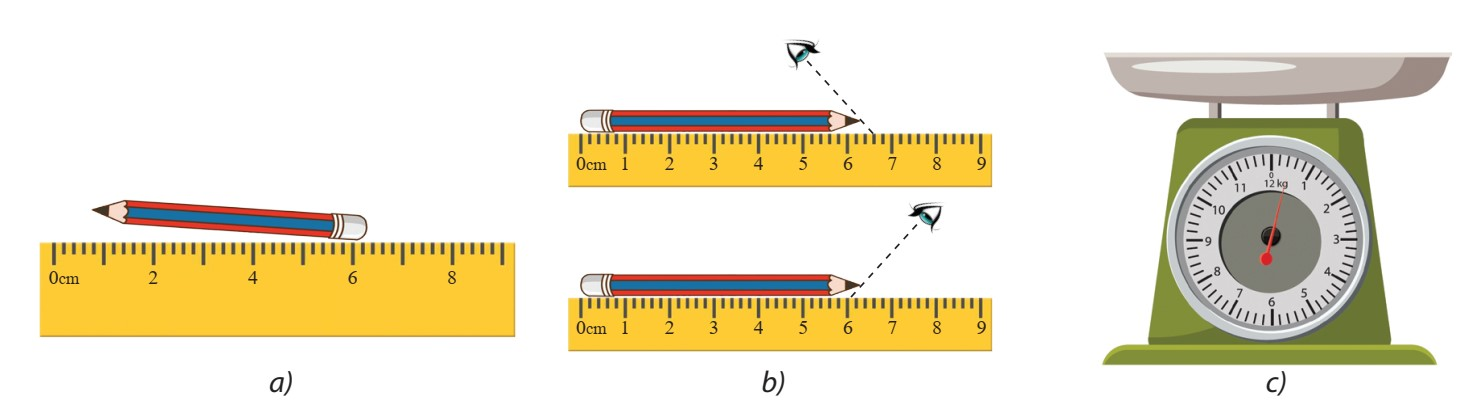
\includegraphics[scale=0.5]{figs/G10Y25B2-1}
		\end{center}
		\loigiai{
			\begin{enumerate}[label=\alph*)]
				\item Đặt bút không dọc theo thước, đầu bút không trùng với vạch số 0.
				\item Đặt mắt sai cách, hướng nhìn không vuông góc.
				\item Kim cân chưa được hiệu chỉnh về số 0.
			\end{enumerate}
		}
	\end{vd}
\begin{dang}{Vận dụng mối liên hệ giữa đơn vị dẫn xuất với 7 đơn vị cơ bản của hệ SI}
\end{dang}
\begin{vd}
	Để xác định quãng đường đi được $s$ của một chất điểm chuyển động thẳng đều, một bạn học sinh đã viết công thức như sau: $s=\alpha\cdot v\cdot t^2$ với $v$ và $t$ lần lượt là vận tốc và thời gian, $\alpha$ là hằng số không thứ nguyên. Dựa vào việc xác định thứ nguyên, em hãy cho biết công thức trên là đúng hay sai.
	\loigiai{
		Thứ nguyên của các đại lượng $s$, $v$ và $t$ lần lượt là
		\begin{itemize}
			\item $\left[s\right]=L$
			\item $\left[v\right]=L\cdot T^{-1}$
			\item $\left[t\right]=T$
		\end{itemize}
		Từ đó, ta thấy vế trái của công thức trên có thứ nguyên $L$ trong khi vế phải lại có thứ nguyên $L\cdot T$. Do 2 vế của công thức không cùng thứ nguyên nên bạn học sinh chưa đưa ra được công thức chính xác.
		Dựa vào phân tích thứ nguyên, ta cần sửa lại công thức chính xác như sau:
		$$s=\alpha \cdot v\cdot t$$
		Trong hệ SI, $s$, $v$ và $t$ lần lượt có đơn vị là $\si{\meter}, \si{\meter\cdot\second^{-1}}, \si{\second}$.
	}
\end{vd}
\begin{dang}{Xác định được sai số tuyệt đối, sai số tỉ đối và biểu diễn được kết quả đo}
\end{dang}
\begin{vd}
	Cho bảng số liệu thể hiện kết quả đo đường kính của một viên bi thép bằng thước kẹp có sai số dụng cụ là $\SI{0.02}{\milli\meter}$. Tính sai số tuyệt đối, sai số tương đối của phép đo và biểu diễn kết quả đo có kèm theo sai số
	\begin{longtable}{|c|c|c|}
		\hline
		\thead{Lần đo} & \thead{$d \left(\si{\milli\meter}\right)$} & \thead{$\Delta d \left(\si{\milli\meter}\right)$}\\
		\hline
		1 & 6,32 & \dots\\
		\hline
		2 & 6,32 & \dots\\
		\hline
		3 & 6,32 & \dots\\
		\hline
		4 & 6,32 & \dots\\
		\hline
		5 & 6,34 & \dots\\
		\hline
		6 & 6,34 & \dots\\
		\hline
		7 & 6,32 & \dots\\
		\hline
		8 & 6,34 & \dots\\
		\hline
		9 & 6,32 & \dots\\
		\hline
		\textbf{Trung bình} & $\overline{d}=?$ & $\overline{\Delta d}=?$\\
		\hline
	\end{longtable}
	
	\loigiai{
		Giá trị trung bình của đường kính viên bi:
		$$\overline{d}=\dfrac{d_1+d_2+d_3+\dots+d_9}{9}\approx\SI{6.327}{\milli\meter}$$
		Sai số tuyệt đối ứng với mỗi lần đo
		$$\Delta d_i=\left|\overline{d}-d_i\right|$$
		$$\Delta d_1=\Delta d_2=\Delta d_3=\Delta d_4=\Delta d_7=\Delta d_9=\left|\SI{6.327}{\milli\meter}-\SI{6.32}{\milli\meter}\right|=\SI{0.007}{\milli\meter}$$
		$$\Delta d_5=\Delta d_6=\Delta d_8=\left|\SI{6.327}{\milli\meter}-\SI{6.34}{\milli\meter}\right|=\SI{0.013}{\milli\meter}$$
		Sai số tuyệt đối trung bình của phép đo:
		$$\overline{\Delta d}=\dfrac{\Delta d_1+\Delta d_2+\dots+\Delta d_9}{9}=\SI{0.009}{\milli\meter}$$
		Sai số tuyệt đối của phép đo:
		$$\Delta d = \overline{\Delta d}+\Delta d_\text{dc}=\SI{0.009}{\milli\meter}+\SI{0.02}{\milli\meter}=\SI{0.029}{\milli\meter}$$
		Sai số tương đối của phép đo:
		$$\delta d =\dfrac{\Delta d}{\overline{d}}\cdot\SI{100}{\percent}\approx\SI{0.46}{\percent}$$
		Kết quả phép đo:
		$$d=\overline{d}\pm\Delta d=\SI{6.273}{\milli\meter}\pm\SI{0.029}{\milli\meter}.$$
	}
\end{vd}

\begin{vd}
	Trong bài thực hành đo gia tốc trọng trường của Trái Đất tại phòng thí nghiệm, một học sinh đo được chiều dài của con lắc đơn $\ell= \xsi{800\pm 1}{\milli\meter}$ thì chu kì dao động là $T = \xsi{1.78\pm 0.02}{\second}$. Lấy $\pi=\SI{3.14}{}$. Biết chu kỳ của con lắc đơn tính theo công thức $T=2\pi \sqrt{\dfrac{\ell}{g}}$. Gia tốc trọng trường $g$ của Trái Đái tại phòng thí nghiệm đó là bao nhiêu?
	\loigiai{
		Từ công thức: $$T=2\pi \sqrt{\dfrac{\ell}{g}} \Rightarrow g=\dfrac{4\pi^2\ell}{T^2}.$$ 	
		
		Giá trị trung bình của gia tốc trọng trường: 	
		$$\overline{g}=\dfrac{4\pi^2\ell}{T^2}=\dfrac{4\pi^2\cdot \SI{3.14}{}\cdot \SI{0.8}{\meter}}{\left( \SI{1.78}{\second}\right)^2}=\SI{9.96}{\meter\per\second^2}.$$
		
		Sai số tuyệt đối của gia tốc trọng trường:
		\begin{align*}
			\dfrac{\Delta g}{\overline g}&= \dfrac{\Delta \ell}{\overline \ell}+ 2\dfrac{\Delta T}{\overline T}\\
			&=\dfrac{\SI{1}{\milli\meter}}{\SI{800}{\milli\meter}}+2\times\dfrac{\SI{0.02}{\second}}{\SI{1.78}{\second}}\\
			&=\SI{0.024}{}\\
			\Rightarrow\quad \Delta g&= \SI{0.024}{}\cdot \overline g\\
			&= \SI{0.24}{\meter\per\second^2}.
		\end{align*}
		
		
		
		Vậy gia tốc trọng trường của Trái Đất tại phòng thí nghiệm đó là
		$$g={\overline g } \pm \Delta g =\SI{9.96}{\meter\per\second^2}\pm\SI{0.24}{\meter\per\second^2}.$$
	}
\end{vd}

\begin{vd}
	Một học sinh dùng cân và đồng hồ đếm giây để đo độ cứng $k$ của lò xo. Dùng cân để cân vật nặng thu được kết quả khối lượng $m = \SI{100}{\gram}$ với sai số tỉ đối là $\SI{2}{\percent}$. Gắn vật vào lò xo và kích thích cho con lắc dao động rồi dùng đồng hồ đếm giây đo thời gian của một dao động cho kết quả $T = \SI{2}{\second}$ với sai số tỉ đối là $\SI{1}{\percent}$. Biết chu kỳ của con lắc lò xo tính theo công thức $T=2\pi \sqrt{m/k}$. Sai số tỉ đối của phép đo độ cứng của lò xo là bao nhiêu?
	\loigiai{
		Từ công thức: $$T=2\pi \sqrt{\dfrac{m}{k}} \Rightarrow k=\dfrac{4\pi^2m}{T^2}.$$	
		
		Sai số tỉ đối của độ cứng lò xo: 	
		$$\dfrac{\Delta k}{\overline k}= \dfrac{\Delta m}{\overline m}+ 2\dfrac{\Delta T}{\overline T}= \SI{2}{\percent}+2\cdot \SI{1}{\percent}= \SI{4}{\percent}.$$
		
		Vậy sai số tỉ đối của phép đo độ cứng của lò xo là $\SI{4}{\percent}.$
	}
\end{vd}
\subsection{TRẮC NGHIỆM NHIỀU PHƯƠNG ÁN LỰA CHỌN}
\setcounter{ex}{0}
\Opensolutionfile{ans}[ans/G10Y25B2-TN]
\begin{ex}
	Chọn đáp án có từ/cụm từ thích hợp để hoàn thành bảng sau:
	\begin{center}
		\begin{tabular}{|c|c|c|}
			\hline
			\thead{Đơn vị} & \thead{Kí hiệu} & \thead{Đại lượng }\\
			\hline
			kelvin & (1) & (2)\\
			\hline
			ampe & $\si{\ampere}$ & (3)\\
			\hline
			candela & $\si{\candela}$ & (4)\\
			\hline
		\end{tabular}
	\end{center}
	\choice
	{(1) $\si{\kelvin}$; (2) Khối lượng; (3) Cường độ dòng điện; (4) Lượng chất}
	{\True (1) $\si{\kelvin}$; (2) Nhiệt độ; (3) Cường độ dòng điện; (4) Cường độ ánh sáng}
	{(1) $\si{\kelvin}$; (2) Nhiệt độ; (3) Cường độ dòng điện; (4) Lượng chất}
	{(1) $\si{\kelvin}$; (2) Khối lượng; (3) Cường độ dòng điện; (4) Cường độ ánh sáng}
	\loigiai{}
\end{ex}

\begin{ex}
	Đơn vị nào sau đây không thuộc thứ nguyên $L$ [Chiều dài]?
	\choice
	{Dặm}
	{Hải lí}
	{Năm ánh sáng}
	{\True Năm}
	\loigiai{}
\end{ex}

\begin{ex}
	Chọn đáp án có từ/cụm từ thích hợp để hoàn thành các câu sau:
	\begin{itemize}
		\item Các số hạng trong phép cộng (hoặc trừ) phải có cùng (1) \dots và nên chuyển về cùng (2) \dots.
		\item (3) \dots của một biểu thức vật lí phải có cùng thứ nguyên.
	\end{itemize}
	\choice
	{(1) đơn vị; (2) thứ nguyên; (3) Đại lượng}
	{(1) thứ nguyên; (2) đại lượng; (3) Hai vế}
	{(1) đơn vị; (2) đại lượng; (3) Hai vế}
	{\True (1) thứ nguyên; (2) đơn vị; (3) Hai vế}
	\loigiai{}
\end{ex}

\begin{ex}
	Trong hệ đơn vị SI, tốc độ có đơn vị là
	\choice
	{$\si{\kilo\meter/\hour}$}
	{\True $\si{\meter/\second}$}
	{$\si{\text{dặm}/\hour}$}
	{$\si{ft/\second}$}
	\loigiai{}
\end{ex}

\begin{ex}
	Trong các phép đo dưới đây, đâu là phép đo trực tiếp?
	\begin{enumerate}[label=(\arabic*)]
		\item Dùng thước đo chiều cao.
		\item Dùng cân đo cân nặng.
		\item Dùng cân và ca đong đo khối lượng riêng của nước.
		\item Dùng đồng hồ và cột cây số đo tốc độ của người lái xe.
	\end{enumerate}
	\choice
	{\True (1), (2)}
	{(1), (2), (4)}
	{(2), (3), (4)}
	{(2), (4)}
	\loigiai{}
\end{ex}

\begin{ex}
	Đáp án nào sau đây có 1 đơn vị cơ bản và 1 đơn vị dẫn xuất?
	\choice
	{mét, kilogram}
	{\True newton, mol}
	{pascal, joule}
	{candela, kelvin}
	\loigiai{}
\end{ex}

\begin{ex}
	Giá trị nào sau đây có 2 chữ số có nghĩa (CSCN)?
	\choice
	{$\SI{201}{\meter}$}
	{$\SI{0.02}{\meter}$}
	{$\SI{20}{\meter}$}
	{\True $\SI{210}{\meter}$}
	\loigiai{}
\end{ex}

\begin{ex}
	Một bánh xe có bán kính $R=\xsi{10\pm0.5}{\centi\meter}$. Sai số tương đối của chu vi bánh xe là
	\choice
	{$\SI{0.05}{\percent}$}
	{\True $\SI{5}{\percent}$}
	{$\SI{10}{\percent}$}
	{$\SI{25}{\percent}$}
	\loigiai{
		$$\delta R=\dfrac{\Delta R}{\overline{R}}\cdot\SI{100}{\percent}=\SI{5}{\percent}.$$
	}
\end{ex}

\begin{ex}
	Thứ nguyên của vận tốc là
	\choice
	{$LT$}
	{$L^{-1}T$}
	{$L^{-1}T^{-1}$}
	{\True $LT^{-1}$}
	\loigiai{
		\begin{align*}
			v&=\dfrac{s}{t}\\
			\Rightarrow \left[v\right]&=\dfrac{\left[s\right]}{\left[t\right]}=LT^{-1}.
		\end{align*}
	}
\end{ex}

\begin{ex}
	Thứ nguyên của trọng lượng riêng là
	\choice
	{$MLT^{-1}$}
	{$MLT^{-2}$}
	{$ML^{-2}T^{-1}$}
	{\True $ML^{-2}T^{-2}$}
	\loigiai{
		\begin{align*}
			d&=\dfrac{P}{V}\\
			\Rightarrow \left[d\right]&=\dfrac{\left[P\right]}{\left[V\right]}\\
			\Leftrightarrow \left[d\right]&=\dfrac{MLT^{-2}}{L^3}=ML^{-2}T^{-2}.
		\end{align*}
	}
\end{ex}
\Closesolutionfile{ans}
\subsection{TỰ LUẬN VÀ TRẢ LỜI NGẮN}
\setcounter{ex}{0}
\Opensolutionfile{ans}[ans/G10Y25B2-SA]
\begin{ex}
	Một học sinh làm thí nghiệm đo chiều dài của bàn học bằng thước. Sau 6 lần đo, bạn học sinh tính được:
	\begin{itemize}
		\item Giá trị trung bình chiều dài bàn là $\overline{\ell}=\SI{1202}{\milli\meter}$.
		\item Sai số trung bình là $\overline{\Delta\ell}=\SI{2}{\milli\meter}$.
	\end{itemize}
	Biết sai số dụng cụ đo là $\Delta \ell_\text{dc}=\SI{1}{\milli\meter}$.\\
	Bạn hãy trình bày kết quả phép đo của học sinh trên.
	\loigiai{
		Sai số tuyệt đối của phép đo:
		$$\Delta \ell=\overline{\Delta \ell}+\Delta\ell_\text{dc}=\SI{3}{\milli\meter}.$$
		Kết quả phép đo:
		$$\ell=\overline{\ell}\pm\Delta\ell=\xsi{1202\pm3}{\milli\meter}.$$
	}
\end{ex}

\begin{ex}
	Em hãy lập phương án đo tốc độ chuyển động của ô tô đồ chơi, chỉ dùng thước và đồng hồ bấm giây để trả lời các câu hỏi sau:
	\begin{enumerate}[label=\alph*)]
		\item Để đo tốc độ chuyển động của chiếc xe, cần đo những đại lượng nào?
		\item Xác định tốc độ chuyển động của xe theo công thức nào?
		\item Phép đo nào là phép đo trực tiếp? Tại sao?
		\item Phép đo nào là phép đo gián tiếp? Tại sao?
	\end{enumerate}
	\loigiai{	
		\begin{enumerate}[label=\alph*)]
			\item Để đo tốc độ chuyển động của chiếc xe, cần đo những đại lượng: đo quãng đường xe di chuyển được và thời gian xe di chuyển.
			\item Xác định tốc độ chuyển động của xe theo công thức:
			$$v = \dfrac{s}{t}.$$
			\item Phép đo quãng đường và thời gian là phép đo trực tiếp. Vì ta thực hiện động tác trực tiếp lên các dụng cụ thí nghiệm.
			\item Phép đo xác đinh vận tốc là phép đo gián tiếp. Vì phép đo này có được cần phải thông qua hai phép đo kia.
		\end{enumerate}
	}
\end{ex}

\begin{ex}
	Hình \ref{fig:3P-1} thể hiện nhiệt kế đo nhiệt độ $t_1$ $\left(\si{\degree C}\right)$ và $t_2$ $\left(\si{\degree C}\right)$ của một dung dịch trước và sau khi đun. Hãy xác định và ghi kết quả độ tăng nhiệt độ $t$ của dung dịch này.
	\begin{center}
		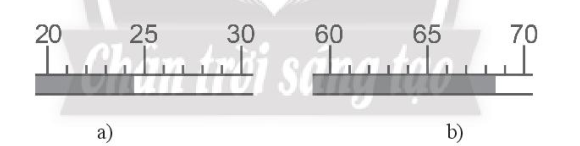
\includegraphics[scale=0.5]{figs/G10Y25B2-2}
		\captionof{figure}{Nhiệt kế: \textit{a) trước; b) sau khi đun dung dịch}}
		\label{fig:3P-1}
	\end{center}
	\loigiai{
		Lấy sai số dụng cụ $\Delta t_\text{dc}=\dfrac{\text{ĐCNN}}{2}=\SI{0.5}{\degree C}$.\\
		Nhiệt độ ban đầu:
		$$t_1=\xsi{24\pm0.5}{\degree C}$$
		Nhiệt độ lúc sau:
		$$t_2=\xsi{68\pm 0.5}{\degree C}$$
		Độ tăng nhiệt độ của dung dịch này:
		$$t=t_2-t_1=\xsi{44.0\pm1.0}{\degree C}.$$
	}
\end{ex}

\begin{ex}
	Hãy xác định số CSCN của các số sau đây: $123,45$; $1,990$; $3,110\cdot 10^{-9}$; $1907,21$; $0,002099$; $12768000$. 
	\loigiai{
		$123,45$ - 5 CSCN; $1,990$ - 4 CSCN; $3,110\cdot10^{-9}$ - 4 CSCN; $1907,21$ - 6 CSCN; $0,002099$ - 4 CSCN; $12768000$ - 5 CSCN.
	}
\end{ex}

\begin{ex}
	Một viên bị hình cầu có bán kính $r$ đang chuyển động với tốc độ $v$ trong dầu. Viên bị chịu tác dụng của lực cản có độ lớn được cho bởi biểu thức $F=c\cdot r\cdot v$, trong đó $c$ là một hằng số. Xác định đơn vị của $c$ theo đơn vị của lực, chiều dài và thời gian trong hệ SI.
	\loigiai{
		Từ công thức trên đề bài $\Rightarrow c=\dfrac{F}{r\cdot v}$\\
		Đơn vị của $c$ là: $\si{\newton\cdot\meter^{-2}\cdot\second}$.
	}
\end{ex}

\begin{ex}
	Một vật có khối lượng $m$ và thể tích $V$, có khối lượng riêng $\rho$ được xác định bằng công thức $\rho =\dfrac{m}{V}$. Biết sai số tương đối của phép đo $m$ và $V$ lần lượt là $\SI{12}{\percent}$ và $\SI{5}{\percent}$. Hãy xác định sai số tương đối của phép đo $\rho$.
	\loigiai{
		$$\delta \rho=\delta m+\delta V=\SI{12}{\percent}+\SI{5}{\percent}=\SI{17}{\percent}.$$
	}
\end{ex}

\begin{ex}
	Một học sinh muốn xác định gia tốc rơi tự do $g$ bằng cách thả một quả bóng từ độ cao $h$ và dùng đồng hồ để bấm thời gian rơi $t$ của quả bóng. Sau đó, thông qua quá trình tìm hiểu, bạn sử dụng công thức $h=\dfrac{1}{2}g\cdot t^2$ để xác định $g$. Hãy nêu ít nhất 2 giải pháp giúp bạn học sinh đó giảm sai số trong quá trình thực nghiệm để thu được kết quả chính xác nhất.
	\loigiai{
		Một số giải pháp phù hợp: hạn chế sự tác động của lực cản không khí, thả rơi quả bóng ở nhiều độ cao khác nhau, sử dụng đồng hồ có độ nhạy cao, thao tác bấm đồng hồ dứt khoát.
	}
\end{ex}

\begin{ex}
	\begin{center}
		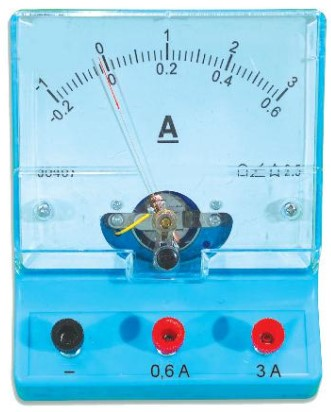
\includegraphics[scale=0.6]{figs/G10Y25B2-3}
	\end{center}
	\begin{enumerate}[label=\alph*)]
		\item Giới hạn đo của ampe kế là bao nhiêu?
		\item Nếu sử dụng ampe kế để đo dòng điện vượt quá giới hạn đo thì có thể gây ra nguy cơ gì?
	\end{enumerate}
	\loigiai{	
		\begin{enumerate}[label=\alph*)]
			\item Giới hạn đo của ampe kế ở hình là $\SI{3}{A}$.
			\item Nếu sử dụng ampe kế để đo dòng điện vượt quá giới hạn đo thì có thể làm cho ampe kế bị hư hỏng.
		\end{enumerate}
	}
\end{ex}

\begin{ex}
	Hãy xác định số đo chiều dài của cây bút chì trong các trường hợp dưới đây:
	\begin{center}
		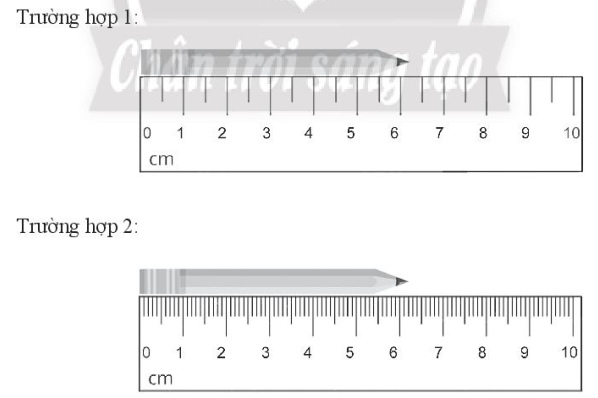
\includegraphics[scale=0.5]{figs/G10Y25B2-4}
	\end{center}
	\loigiai{
		\begin{itemize}
			\item Trường hợp 1: $\ell=\xsi{6.0\pm0.3}{\centi\meter}$.
			\item Trường hợp 2: $\ell=\xsi{6.20\pm0.05}{\centi\meter}$.
		\end{itemize}
	}
\end{ex}

\begin{ex}
	Đo chiều dày của một cuốn sách, được kết quả: $\SI{2.3}{cm}$; $\SI{2.4}{cm}$; $\SI{2.5}{cm}$; $\SI{2.4}{cm}$. Tính giá trị trung bình chiều dày cuốn sách. Sai số tuyệt đối trung bình của phép đo này là bao nhiêu?
	\loigiai{
		Ta có: 
		$$\overline{A} = \dfrac{A_1 + A_2 +...+ A_n}{n} =\SI{2.4}{cm}.$$
		Vậy trung bình chiều dày cuốn sách là $\SI{2.4}{cm}.$
		$$\Delta A_1 = |0.1|.$$
		$$\Delta A_2 = |0|.$$
		$$\Delta A_3 = |0.1|.$$
		$$\Delta A_4 = |0|.$$
		Ta có:
		$$\Delta \overline{A} = \dfrac{\Delta A_1 + \Delta A_2 +\Delta A_3+ \Delta A_4}{4} =\SI{0.05}{cm}.$$
		Vậy sai số tuyệt đối trung bình là $\SI{0.05}{cm}.$
	}
\end{ex}

\begin{ex}
	Bảng ghi thời gian một vật rơi giữa hai điểm cố định:
	\begin{center}
		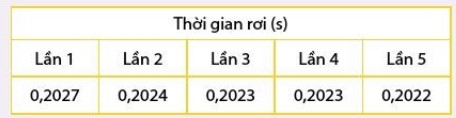
\includegraphics[scale=1]{figs/G10Y25B2-5}
	\end{center}
	\begin{enumerate}[label=\alph*)]
		\item Tính giá trị trung bình của thời gian rơi.
		\item Tìm sai số tuyệt đối trung bình.
	\end{enumerate}
	\loigiai{
		\begin{enumerate}[label=\alph*)]
			\item Giá trị trung bình của thời gian rơi là:
			$$\dfrac{0.2027 + 0.2024+ 0.2023+ 0.2023+ 0.2022}{5} \approx 0.2024$$
			\item Sai số tuyệt đối:
			$$A_1= |0.2024 - 0.2027| = 0.0003.$$
			$$A_2= |0.2024 - 0.2024| = 0.0000.$$
			$$A_3= |0.2024 - 0.2023| = 0.0001.$$
			$$A_4= |0.2024 - 0.2023| = 0.0001.$$
			$$A_5= |0.2024 - 0.2022| = 0.0002.$$
			Sai số tuyệt đối trung bình là: 
			$$\dfrac{0.0003 + 0.0000 + 0.0001 + 0.0001 + 0.0002}{5} = 0.00014.$$
		\end{enumerate}
	}
\end{ex}

\begin{ex}
	Dùng một đồng hồ đo thời gian có độ chia nhỏ nhất là $\SI{0.001}{\second}$ để đo $n$ lần thời gian rơi tự do của một vật bắt đầu từ điểm A đến điểm B. Kết quả đo hiển thị trong bảng sau:
	\begin{center}
		\begin{tabular}{|C{5em}|C{5em}|C{5em}|}
			\hline
			\thead{n} & \thead{\xsi{t}{\left(\second\right)}} &\thead{$\Delta t_i$}\\
			\hline
			1 & 0,398 &\\
			\hline
			2 & 0,399 &\\
			\hline
			3 & 0,408 & \\
			\hline
			4 & 0,410 &\\
			\hline
			5 & 0,406&\\
			\hline
			6 & 0,405 &\\
			\hline
			\thead{Trung bình} & &\\
			\hline
		\end{tabular}
	\end{center}
	Hãy tính thời gian rơi trung bình, sai số ngẫu nhiên, sai số dụng cụ và sai số phép đo thời gian. Phép đo này là phép đo trực tiếp hay gián tiếp?
	\loigiai{
		\begin{center}
			\begin{tabular}{|C{5em}|C{5em}|C{5em}|}
				\hline
				\thead{n} & \thead{\xsi{t}{\left(\second\right)}} &\thead{$\Delta t_i$}\\
				\hline
				1 & 0,398 & 0,0063\\
				\hline
				2 & 0,399 &0,0053\\
				\hline
				3 & 0,408 & 0,0037\\
				\hline
				4 & 0,410 &0,0057\\
				\hline
				5 & 0,406&0,0017\\
				\hline
				6 & 0,405 &0,0007\\
				\hline
				\thead{Trung bình} &0,4043 &0,0039\\
				\hline	
			\end{tabular}
		\end{center}
		\begin{itemize}
			\item Thời gian rơi trung bình: $\overline{t}=\SI{0.4043}{\second}$.
			\item Sai số dụng cụ: $\Delta t_\text{dc}=\dfrac{\text{ĐCNN}}{2}=\SI{0.0005}{\second}$.
			\item Sai số ngẫu nhiên: $\overline{\Delta t}=\SI{0.0039}{\second}$.
			\item Sai số phép đo thời gian: $\Delta t=\overline{\Delta t}+\Delta t_\text{dc}=\SI{0.0044}{\second}$.
		\end{itemize}
	}
\end{ex}

\begin{ex}
	Dùng thước kẹp có ĐCNN $\SI{0.1}{mm}$ để đo 5 lần đường kính $d$ và chiều cao $h$ của một trụ thép, cho kết quả như trong bảng sau:
	\begin{center}
		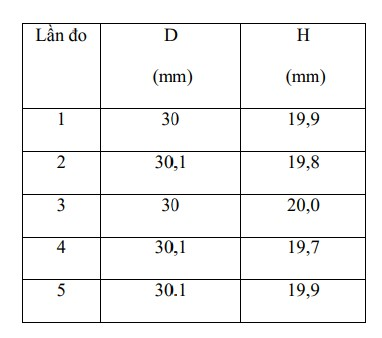
\includegraphics[scale=1]{figs/G10Y25B2-6}
	\end{center}
	Hãy cho biết kết quả phép đo $d, h$ và tính thể tích trụ thép.
	\loigiai{	
		Phép đo $d, h$ là phép đo trực tiếp, giá trị
		trung bình và sai số ngẫu nhiên tính trong
		bảng sau
		\begin{center}
			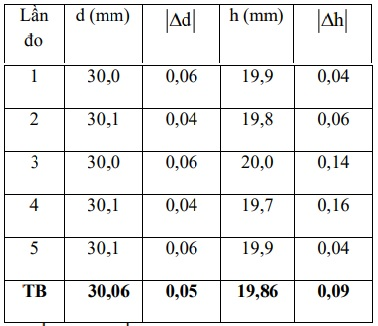
\includegraphics[scale=1]{figs/G10Y25B2-7}
		\end{center}
		Sai số dụng cụ bằng $\SI{0.1}{mm}$. Vậy:
		Sai số phép đo đường kính trụ là:
		$$\Delta d = 0.05 + 0.05 =\SI{0.10}{mm}.$$
		Sai số phép đo chiều cao trụ là:
		$$\Delta h = 0.09 + 0.05 =\SI{0.14}{mm}.$$
		Kết quả: 
		$$d = \xsi{30.06\pm0.10}{\milli\meter}.$$
		$$h = \xsi{19.86\pm0.14}{\milli\meter}.$$
		Thể tích trung bình của khối trụ:
		$$\overline{V} = \dfrac{\pi \overline{d}^2 \overline{h}}{4} =\SI{14094.42}{\cubic\milli\meter}.$$
		Sai số tỉ đối:
		$$\dfrac{\Delta V}{\overline V} = 2 \dfrac{\overline{\Delta d}}{\overline d} + \dfrac{\overline {\Delta h}}{\overline{h}} + \dfrac{\Delta \pi}{\pi} = 0.014 = \SI{1.4}{\percent}.$$
		Sai số tuyệt đối:
		$$\Delta V = \overline{V} \cdot \delta V = \SI{193.13}{\cubic\milli\meter}.$$
		Suy ra:
		$$V = \xsi{14094\pm193}{\cubic\milli\meter}.$$
	}
\end{ex}
\Closesolutionfile{ans}